\section{Formulate Statement}

\subsection{ Redefinition of Narrow RevTerminate Principle}
相較於 informal logic proof, we need 更嚴格的定義 for our formal logic proof.
Here is the Narrow RevTerminate Principle:
``Given a reversible abstract machine with a finite number of total states, it will inevitably terminate from any initial state.''

First of all, we define the initial state.  Given a state, if 他不是任何state的next state,we call the state is initial.
\begin{code}%
\>[2]\AgdaFunction{is-initial} %
\AgdaSymbol{:} %
\AgdaField{State} %
\AgdaSymbol{→} %
\AgdaPrimitive{Set} %
\AgdaSymbol{\AgdaUnderscore{}}\<%
\\
%
\>[2]\AgdaFunction{is-initial} %
\AgdaBound{st} %
\AgdaSymbol{=} %
\AgdaFunction{∄[} %
\AgdaBound{st'} %
\AgdaFunction{]} %
\AgdaSymbol{(}\AgdaBound{st'} %
\AgdaOperator{\AgdaField{↦}} %
\AgdaBound{st}\AgdaSymbol{)}\<%
\\
\>[0]\<%
\end{code}

Secondly, we define the terminate of a reversible machine.
Starting from the initial state $st_{0}$, we use $st_{0}$ $\mapsto$* $st_{n}$ presents $st_{0}$ can reach $st_{n}$ by walk through finite steps.
\begin{code}%
    \>[2]\AgdaKeyword{data} %
    \AgdaOperator{\AgdaDatatype{\AgdaUnderscore{}↦*\AgdaUnderscore{}}} %
    \AgdaSymbol{:} %
    \AgdaField{State} %
    \AgdaSymbol{→} %
    \AgdaField{State} %
    \AgdaSymbol{→} %
    \AgdaPrimitive{Set} %
    \AgdaSymbol{(}\AgdaPrimitive{L.suc} %
    \AgdaBound{ℓ}\AgdaSymbol{)} %
    \AgdaKeyword{where}\<%
    \\
    \>[2][@{}l@{\AgdaIndent{0}}]%
    \>[4]\AgdaInductiveConstructor{◾} %
    \AgdaSymbol{:} %
    \AgdaSymbol{\{}\AgdaBound{st} %
    \AgdaSymbol{:} %
    \AgdaField{State}\AgdaSymbol{\}} %
    \AgdaSymbol{→} %
    \AgdaBound{st} %
    \AgdaOperator{\AgdaDatatype{↦*}} %
    \AgdaBound{st}\<%
    \\
    %
    \>[4]\AgdaOperator{\AgdaInductiveConstructor{\AgdaUnderscore{}∷\AgdaUnderscore{}}} %
    \AgdaSymbol{:} %
    \AgdaSymbol{\{}\AgdaBound{st₁} %
    \AgdaBound{st₂} %
    \AgdaBound{st₃} %
    \AgdaSymbol{:} %
    \AgdaField{State}\AgdaSymbol{\}} %
    \AgdaSymbol{→} %
    \AgdaBound{st₁} %
    \AgdaOperator{\AgdaField{↦}} %
    \AgdaBound{st₂} %
    \AgdaSymbol{→} %
    \AgdaBound{st₂} %
    \AgdaOperator{\AgdaDatatype{↦*}} %
    \AgdaBound{st₃} %
    \AgdaSymbol{→} %
    \AgdaBound{st₁} %
    \AgdaOperator{\AgdaDatatype{↦*}} %
    \AgdaBound{st₃}\<%
    \\
    \>[0]\<%
\end{code}

And if a state $st_{0}$ have no next state, we call the state is stuck.
\begin{code}%
\>[2]\AgdaFunction{is-stuck} %
\AgdaSymbol{:} %
\AgdaField{State} %
\AgdaSymbol{→} %
\AgdaPrimitive{Set} %
\AgdaSymbol{\AgdaUnderscore{}}\<%
\\
%
\>[2]\AgdaFunction{is-stuck} %
\AgdaBound{st} %
\AgdaSymbol{=} %
\AgdaFunction{∄[} %
\AgdaBound{st'} %
\AgdaFunction{]} %
\AgdaSymbol{(}\AgdaBound{st} %
\AgdaOperator{\AgdaField{↦}} %
\AgdaBound{st'}\AgdaSymbol{)}\<%
\\
\>[0]\<%
\end{code}

The terminate of a reversible machine means ``given an initial state, it will reach a stuck state.''
\begin{code}%
\>[2]\AgdaFunction{is-stuck} %
\AgdaSymbol{:} %
\AgdaField{State} %
\AgdaSymbol{→} %
\AgdaPrimitive{Set} %
\AgdaSymbol{\AgdaUnderscore{}}\<%
\\
%
\>[2]\AgdaFunction{is-stuck} %
\AgdaBound{st} %
\AgdaSymbol{=} %
\AgdaFunction{∄[} %
\AgdaBound{st'} %
\AgdaFunction{]} %
\AgdaSymbol{(}\AgdaBound{st} %
\AgdaOperator{\AgdaField{↦}} %
\AgdaBound{st'}\AgdaSymbol{)}\<%
\\
\>[0]\<%
\end{code}

At last, we define ``a reversible abstract machine with finite number of total states.''
Here is the definition of Fin in agda.  a Fin N set have exactly N elements.
\begin{code}%
\>[2]\AgdaFunction{is-stuck} %
\AgdaSymbol{:} %
\AgdaField{State} %
\AgdaSymbol{→} %
\AgdaPrimitive{Set} %
\AgdaSymbol{\AgdaUnderscore{}}\<%
\\
%
\>[2]\AgdaFunction{is-stuck} %
\AgdaBound{st} %
\AgdaSymbol{=} %
\AgdaFunction{∄[} %
\AgdaBound{st'} %
\AgdaFunction{]} %
\AgdaSymbol{(}\AgdaBound{st} %
\AgdaOperator{\AgdaField{↦}} %
\AgdaBound{st'}\AgdaSymbol{)}\<%
\\
\>[0]\<%
\end{code}

We construct a bijection relation between state and Fin N.
It seems like all states are indexed by one of element in Fin N set.
\begin{code}%
\>[2]\AgdaFunction{is-stuck} %
\AgdaSymbol{:} %
\AgdaField{State} %
\AgdaSymbol{→} %
\AgdaPrimitive{Set} %
\AgdaSymbol{\AgdaUnderscore{}}\<%
\\
%
\>[2]\AgdaFunction{is-stuck} %
\AgdaBound{st} %
\AgdaSymbol{=} %
\AgdaFunction{∄[} %
\AgdaBound{st'} %
\AgdaFunction{]} %
\AgdaSymbol{(}\AgdaBound{st} %
\AgdaOperator{\AgdaField{↦}} %
\AgdaBound{st'}\AgdaSymbol{)}\<%
\\
\>[0]\<%
\end{code}

Combine the definition above, and we have the exact definition of Narrow RevTerminate Principle:
\begin{code}%
    \>[2]\AgdaFunction{Finite-State-Termination} %
    \AgdaSymbol{:} %
    \AgdaSymbol{∀} %
    \AgdaSymbol{\{}\AgdaBound{N} %
    \AgdaBound{st₀}\AgdaSymbol{\}}\<%
    \\
    \>[2][@{}l@{\AgdaIndent{0}}]%
    \>[4]\AgdaSymbol{→} %
    \AgdaField{State} %
    \AgdaOperator{\AgdaFunction{⤖}} %
    \AgdaDatatype{Fin} %
    \AgdaBound{N}\<%
    \\
    %
    \>[4]\AgdaSymbol{→} %
    \AgdaSymbol{(}\AgdaBound{has-next} %
    \AgdaSymbol{:} %
    \AgdaSymbol{∀} %
    \AgdaSymbol{(}\AgdaBound{st} %
    \AgdaSymbol{:} %
    \AgdaField{State}\AgdaSymbol{)} %
    \AgdaSymbol{→} %
    \AgdaRecord{Dec} %
    \AgdaSymbol{(}\AgdaFunction{∃[} %
    \AgdaBound{st'} %
    \AgdaFunction{]} %
    \AgdaSymbol{(}\AgdaBound{st} %
    \AgdaOperator{\AgdaField{↦}} %
    \AgdaBound{st'}\AgdaSymbol{)))}\<%
    \\
    %
    \>[4]\AgdaSymbol{→} %
    \AgdaFunction{is-initial} %
    \AgdaBound{st₀}\<%
    \\
    %
    \>[4]\AgdaSymbol{→} %
    \AgdaFunction{∃[} %
    \AgdaBound{stₙ} %
    \AgdaFunction{]} %
    \AgdaSymbol{(}\AgdaBound{st₀} %
    \AgdaOperator{\AgdaDatatype{↦*}} %
    \AgdaBound{stₙ} %
    \AgdaOperator{\AgdaFunction{×}} %
    \AgdaFunction{is-stuck} %
    \AgdaBound{stₙ}\AgdaSymbol{)}\<%
    \\
    \>[0]\<%
\end{code}

\subsection{ Redefinition of Broad RevTerminate Principle}
Here is the Broad RevTerminate Principle:
``Given a reversible abstract machine, it will inevitably terminate from any initial state with a finite number of reachable states.''

Most of the definitions are same as Narrow RevTerminate Principle, we have:

Given $st_{0}$.  For all of the states, if their next state is not $st_{0}$, then $st_{0}$ is initial state.
\begin{code}%
\>[2]\AgdaFunction{is-initial} %
\AgdaSymbol{:} %
\AgdaField{State} %
\AgdaSymbol{→} %
\AgdaPrimitive{Set} %
\AgdaSymbol{\AgdaUnderscore{}}\<%
\\
%
\>[2]\AgdaFunction{is-initial} %
\AgdaBound{st} %
\AgdaSymbol{=} %
\AgdaFunction{∄[} %
\AgdaBound{st'} %
\AgdaFunction{]} %
\AgdaSymbol{(}\AgdaBound{st'} %
\AgdaOperator{\AgdaField{↦}} %
\AgdaBound{st}\AgdaSymbol{)}\<%
\\
\>[0]\<%
\end{code}

$st_{0}$ $\mapsto$* $st_{n}$ presents $st_{0}$ can reach $st_{n}$ by walk through finite steps.
\begin{code}%
    \>[2]\AgdaKeyword{data} %
    \AgdaOperator{\AgdaDatatype{\AgdaUnderscore{}↦*\AgdaUnderscore{}}} %
    \AgdaSymbol{:} %
    \AgdaField{State} %
    \AgdaSymbol{→} %
    \AgdaField{State} %
    \AgdaSymbol{→} %
    \AgdaPrimitive{Set} %
    \AgdaSymbol{(}\AgdaPrimitive{L.suc} %
    \AgdaBound{ℓ}\AgdaSymbol{)} %
    \AgdaKeyword{where}\<%
    \\
    \>[2][@{}l@{\AgdaIndent{0}}]%
    \>[4]\AgdaInductiveConstructor{◾} %
    \AgdaSymbol{:} %
    \AgdaSymbol{\{}\AgdaBound{st} %
    \AgdaSymbol{:} %
    \AgdaField{State}\AgdaSymbol{\}} %
    \AgdaSymbol{→} %
    \AgdaBound{st} %
    \AgdaOperator{\AgdaDatatype{↦*}} %
    \AgdaBound{st}\<%
    \\
    %
    \>[4]\AgdaOperator{\AgdaInductiveConstructor{\AgdaUnderscore{}∷\AgdaUnderscore{}}} %
    \AgdaSymbol{:} %
    \AgdaSymbol{\{}\AgdaBound{st₁} %
    \AgdaBound{st₂} %
    \AgdaBound{st₃} %
    \AgdaSymbol{:} %
    \AgdaField{State}\AgdaSymbol{\}} %
    \AgdaSymbol{→} %
    \AgdaBound{st₁} %
    \AgdaOperator{\AgdaField{↦}} %
    \AgdaBound{st₂} %
    \AgdaSymbol{→} %
    \AgdaBound{st₂} %
    \AgdaOperator{\AgdaDatatype{↦*}} %
    \AgdaBound{st₃} %
    \AgdaSymbol{→} %
    \AgdaBound{st₁} %
    \AgdaOperator{\AgdaDatatype{↦*}} %
    \AgdaBound{st₃}\<%
    \\
    \>[0]\<%
\end{code}

If a state have no next state, we call the state is stuck.
\begin{code}%
\>[2]\AgdaFunction{is-stuck} %
\AgdaSymbol{:} %
\AgdaField{State} %
\AgdaSymbol{→} %
\AgdaPrimitive{Set} %
\AgdaSymbol{\AgdaUnderscore{}}\<%
\\
%
\>[2]\AgdaFunction{is-stuck} %
\AgdaBound{st} %
\AgdaSymbol{=} %
\AgdaFunction{∄[} %
\AgdaBound{st'} %
\AgdaFunction{]} %
\AgdaSymbol{(}\AgdaBound{st} %
\AgdaOperator{\AgdaField{↦}} %
\AgdaBound{st'}\AgdaSymbol{)}\<%
\\
\>[0]\<%
\end{code}

Before defining ``a finite number of reachable states'', we have to dealt with the ``set of reachable states.''
$st_{0}$ $\mapsto$[m] $st_{m}$ means $st_{0}$ walk exactly m steps and reach $st_{m}$
For all the m and 對應的 $st_{m}$ 滿足 $st_{0}$ $\mapsto$[m] $st_{m}$, it's called ``set of reachable states.''
\begin{code}%
    \AgdaFunction{∃[} %
    \AgdaBound{m} %
    \AgdaFunction{]} %
    \AgdaFunction{∃[} %
    \AgdaBound{stₘ} %
    \AgdaFunction{]} %
    \AgdaSymbol{(}\AgdaBound{st₀} %
    \AgdaOperator{\AgdaDatatype{↦[}} %
    \AgdaBound{m} %
    \AgdaOperator{\AgdaDatatype{]}} %
    \AgdaBound{stₘ}\AgdaSymbol{)} %
    \\
    \>[0]\<%
\end{code}

In agda, each elements of reachable states set seems like a tuple. 
\vspace{1em}

\usetikzlibrary{graphs, positioning, quotes, shapes.geometric}

\begin{document}
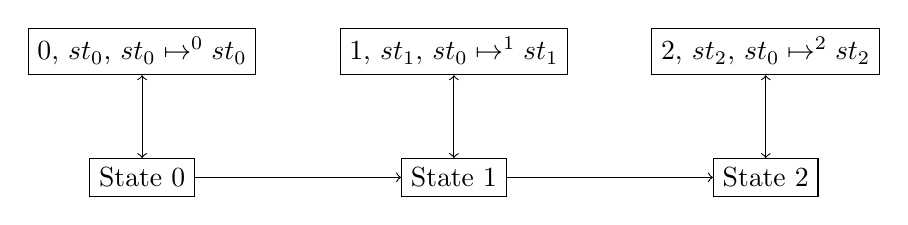
\begin{tikzpicture}[node distance=10pt]
    \node[draw] (Description 0)  {0, $st_{0}$, $st_{0}\mapsto^{0}st_{0}$};
    \node[draw, right=30pt of Description 0] (Description 1)  {1, $st_{1}$, $st_{0}\mapsto^{1}st_{1}$};
    \node[draw, right=30pt of Description 1] (Description 2)  {2, $st_{2}$, $st_{0}\mapsto^{2}st_{2}$};
    
    \node[draw, below=30pt of Description 0]    (State 0)  {State 0};
    \node[draw, below=30pt of Description 1]    (State 1)  {State 1};
    \node[draw, below=30pt of Description 2]    (State 2)  {State 2};
    

    \graph{
        (State 0) -> (State 1) -> (State 2);
        (State 0) <-> (Description 0);
        (State 1) <-> (Description 1);
        (State 2) <-> (Description 2);
    };
\end{tikzpicture}

Then, we construct a bijection relation between reachable state set and Fin N.
\begin{code}%
    \AgdaBound{St-Fin} %
    \AgdaSymbol{:} %
    \AgdaFunction{∃[} %
    \AgdaBound{m} %
    \AgdaFunction{]} %
    \AgdaFunction{∃[} %
    \AgdaBound{stₘ} %
    \AgdaFunction{]} %
    \AgdaSymbol{(}\AgdaBound{st₀} %
    \AgdaOperator{\AgdaDatatype{↦[}} %
    \AgdaBound{m} %
    \AgdaOperator{\AgdaDatatype{]}} %
    \AgdaBound{stₘ}\AgdaSymbol{)} %
    \AgdaOperator{\AgdaFunction{⤖}} %
    \AgdaDatatype{Fin} %
    \AgdaBound{N}\<%
    \\
\end{code}

It seems like all reachable states are indexed by one of element in Fin N set.
\begin{code}%
    \AgdaBound{St-Fin} %
    \AgdaSymbol{:} %
    \AgdaFunction{∃[} %
    \AgdaBound{m} %
    \AgdaFunction{]} %
    \AgdaFunction{∃[} %
    \AgdaBound{stₘ} %
    \AgdaFunction{]} %
    \AgdaSymbol{(}\AgdaBound{st₀} %
    \AgdaOperator{\AgdaDatatype{↦[}} %
    \AgdaBound{m} %
    \AgdaOperator{\AgdaDatatype{]}} %
    \AgdaBound{stₘ}\AgdaSymbol{)} %
    \AgdaOperator{\AgdaFunction{⤖}} %
    \AgdaDatatype{Fin} %
    \AgdaBound{N}\<%
    \\
\end{code}

Combine the definition above, and we have the exact definition of Narrow RevTerminate Principle:
\begin{code}%
    \>[2]\AgdaFunction{Finite-Reachable-State-Termination} %
    \AgdaSymbol{:} %
    \AgdaSymbol{∀} %
    \AgdaSymbol{\{}\AgdaBound{N} %
    \AgdaBound{st₀}\AgdaSymbol{\}}\<%
    \\
    \>[2][@{}l@{\AgdaIndent{0}}]%
    \>[4]\AgdaSymbol{→} %
    \AgdaSymbol{(}\AgdaBound{St-Fin} %
    \AgdaSymbol{:} %
    \AgdaFunction{∃[} %
    \AgdaBound{m} %
    \AgdaFunction{]} %
    \AgdaFunction{∃[} %
    \AgdaBound{stₘ} %
    \AgdaFunction{]} %
    \AgdaSymbol{(}\AgdaBound{st₀} %
    \AgdaOperator{\AgdaDatatype{↦[}} %
    \AgdaBound{m} %
    \AgdaOperator{\AgdaDatatype{]}} %
    \AgdaBound{stₘ}\AgdaSymbol{)} %
    \AgdaOperator{\AgdaFunction{⤖}} %
    \AgdaDatatype{Fin} %
    \AgdaBound{N}\AgdaSymbol{)}\<%
    \\
    %
    \>[4]\AgdaSymbol{→} %
    \AgdaSymbol{(}\AgdaBound{has-next} %
    \AgdaSymbol{:} %
    \AgdaSymbol{∀} %
    \AgdaSymbol{(}\AgdaBound{st} %
    \AgdaSymbol{:} %
    \AgdaField{State}\AgdaSymbol{)} %
    \AgdaSymbol{→} %
    \AgdaRecord{Dec} %
    \AgdaSymbol{(}\AgdaFunction{∃[} %
    \AgdaBound{st'} %
    \AgdaFunction{]} %
    \AgdaSymbol{(}\AgdaBound{st} %
    \AgdaOperator{\AgdaField{↦}} %
    \AgdaBound{st'}\AgdaSymbol{)))}\<%
    \\
    %
    \>[4]\AgdaSymbol{→} %
    \AgdaFunction{is-initial} %
    \AgdaBound{st₀}\<%
    \\
    %
    \>[4]\AgdaSymbol{→} %
    \AgdaFunction{∃[} %
    \AgdaBound{stₙ} %
    \AgdaFunction{]} %
    \AgdaSymbol{(}\AgdaBound{st₀} %
    \AgdaOperator{\AgdaDatatype{↦*}} %
    \AgdaBound{stₙ} %
    \AgdaOperator{\AgdaFunction{×}} %
    \AgdaFunction{is-stuck} %
    \AgdaBound{stₙ}\AgdaSymbol{)}\<%
    \\
\end{code}







With the steps in informal logic proof, we can construct a Similar proof for the formal one.  However, there are 許多細節需要更詳細的定義.
The 大致上的 steps are shown below:
\begin{enumerate}[1.]
\item Starting from initial state, try looking for its next state. 
\item If the next state exists, keep looking for 再下一個 state
\item Upon reaching the n-th state, proof that it's impossible for the existence of next states with no-repeat principle.
\end{enumerate}.

\subsection{ Countdown rules }
The principle called Finite-State-Termination-Principle, {TODO: 連結到上面3.1的定義}, agda 無法認知 a proof with "proved n case, and any case should be 推導到 the n-th case", but 這樣的證明方式其實是數學歸納法的一個變體,我們引入countdown variable來轉換成normal 數學歸納法:

\input{agdaCode/4.1-narrow-revTermination-with-countdown}
And our target Principle can be regarded as the special case when Countdown is N, 也就是剛開始的時候。

The Countdown 的運作規則 is as below:
\input{agdaCode/4.1-cd-1-system}

To maintain the Countdown, there are cd and m variable.  cd and m is 相對的, and their sum is always be N.  Starting when m is zero and Countdown is N, after a steps, m 將會 increasing and countdown is decreasing.  We use cd-1 principle to ensure the 不變 of the sum.

\subsection{ Termination rules }
The 中途停止的規則:
We have N different states in a RevMachine, but 並不保證given $st_{0}$ can reach any states in RevMachine.  Here is an instance: 

\input{agdaImages/4.1-halfway-hault-image}

In this example, we have 7 steps in total.  Given a initial state State 0, it will just go 2 steps and reach a stuck state rather than the all 6 steps however.

Therefore, the principle 的證明有兩個終止規則:
\begin{enumerate}[1.]
    \item trying to 推進 next step.  However, there is no next step.  In this case we directly got stuck-state. 
    \item trying to 推進 next step until reaching n-th step, and we use no-repeat to 間接地 proof the n-th step should be stuck.
\end{enumerate}.
The former case is much simplier because it 完全地 find what we need. 
And the latter case, we have to keep discussing in the 之後的 sections.

\subsection{ When we are at n-th state }

With the countdown system and 中途停止的規則, we can 專注於處理以下 principle:
When an initial state 經過 n step and reach n-th state, then the n-th state should be stuck.
The formal principle is shown below:

\input{agdaCode/4.1-nth-state-termination-statement}


The proof of 「當抵達 n-th state 會終止」 can be simply分為 the two steps below:
\begin{enumerate}[1.]
    \item 假定n+1-th state存在, with Piegonhole principle ,可以在 n 個 state 映射到 n + 1 個state,而找到重複經過的兩個相同state
    \item No-repeat 告訴我們找到的兩個state不該是相同的,因為他們的step不同,得到矛盾。
\end{enumerate}.

Before introducing Piegonhole principle and No-Repeat Principle, we will discussing mapping rules.

\subsection{ mapping rules }
// TODO: Fin 相關的說明應該都改為 Index
In our proof of n-th Termination case, a critical part is the mapping rules.
We have,
\begin{enumerate}[1.]
    \item an injection from Step to State.  Note that the 定義域 of step is from 0 to N(included both sides)
    \item bijection between State and Index. because of the limitation of States, we should have n indexes in total.
    \item we can also construct an injection from Step to Index easily.  Just Through the two injection and bijection above.
\end{enumerate}.
Here is an 示意圖 for the relations
\input{agdaImages/4.1-mapping-relation}

Note again that there are only n indexes in the relations.
With the relation, we can 更清楚地描述 the Termination proof at n-th state:
\begin{enumerate}[1.]
    \item first of all, we have n+1 states (from $st_{0}$ to $st_{n}$)
    \item with injection from Step to index, we get two different steps mapping to same index using Piegonhole Principle
    \item with bijection from index back to State, the same indexes should be mapped to same states.
    \item No-repeat principle told us that the two different steps should be mapped to different states, and the contradiction occurs.
\end{enumerate}.

\subsection{ Piegonhole principle }
The definition of Piegonhole principle in agda is shown below:

\input{agdaCode/4.1-piegonhole-principle}

The two necessary inputs are 
\begin{enumerate}[1.]
    \item N to N function. In this case, it is the injection from Step to Index. 
    \item all mapped N should be less than N.  The proof is 隱含在 Fin的定義裡面.  That is, a natrual number value of Fin N is always less than N.
\end{enumerate}.

And we could get two different steps which will injection to the same index.

\subsection{ No Repeat }
The definition of No-Repeat-Principle in agda is shown below:

No-Repeat-Principle is proved by {TODO: 學長論文}.  In the principle, we know that the two states with different steps from initial state, they should be different states.
\input{agdaCode/4.1-no-repeat-principle}

// TODO: 可能需要小結論

